\subsection{Administración de Requerimientos - Mantener conectadas las necesidades y el producto [Pendientes: 1. Consolidar los objetivos y requisitos a partir del VFP. 2. Definir los participantes, responsabilidades, autoridad de aprobación y momentos de revisión de cambios. 3. Elaborar un diagrama BPMN que represente el proceso de administración de requerimientos y la creación o actualización de sus artefactos.]}\label{sec:spmp-10-1}
La adaptación de ISO/IEC/IEEE 29148 contempla una especificación de requisitos que se mantiene actualizada durante el desarrollo del proyecto, una matriz de trazabilidad y un registro de cambios para conservar el origen, las características y las comprobaciones de los requisitos~\cite{std29148}. Las necesidades identificadas en entrevistas y en la propuesta del proyecto (VFP) se vinculan directamente con el objetivo general y los objetivos específicos del proyecto (definidos en la sección \ref{sec:spmp-6-2}), asegurando que las funciones del producto —como la consulta de la biblioteca de escenarios FDS, la ingesta meteorológica mediante Open-Meteo y la visualización en Smokeview— respondan de manera trazable al propósito de apoyar al comandante o coordinador de la operación en Aguas Claras~\cite{vfp2026,adaptacion2026,std29148}. Las necesidades identificadas se distinguen de las funciones incorporadas al alcance, de modo que una recomendación conserve su procedencia sin convertirse automáticamente en un compromiso de implementación~\cite{adaptacion2026,std29148}.

ISO/IEC/IEEE 29148 orienta la evaluación del impacto, la revisión y la aprobación de los cambios, junto con la conservación de la trazabilidad y de las versiones. Los momentos de revisión de cambios se establecen de forma periódica durante las revisiones de iteración y de manera puntual cuando se detecten incidencias o ajustes en las fuentes de datos o restricciones de ejecución. La autoridad de aprobación de los cambios corresponde de manera conjunta al director del proyecto y al equipo de trabajo. En el proyecto, estas prácticas se aplicarán a los requisitos de la aplicación y de su biblioteca de escenarios mediante el siguiente procedimiento~\cite{std29148}:
\begin{enumerate}
\item \textbf{Detectar y reportar la necesidad.} La revisión de entrevistas y del VFP, las pruebas y la evaluación con usuarios pueden revelar necesidades nuevas, errores o ajustes de los requisitos. La propuesta se comunicará al equipo y se incorporará al registro de cambios, identificando el requisito afectado, su origen, la justificación y la modificación solicitada.
\item \textbf{Evaluar el impacto.} La matriz de trazabilidad permitirá localizar los requisitos relacionados, componentes y casos de prueba afectados. Se examinarán la claridad, coherencia, viabilidad y posibilidad de comprobar el requisito propuesto, junto con sus efectos sobre el alcance, el esfuerzo, los recursos, la calendarización y la calidad del producto.
\item \textbf{Decidir y registrar.} La revisión de la propuesta conducirá a su aprobación o rechazo por parte de la autoridad de aprobación, conservando la decisión y su justificación en el registro de cambios. La discusión se apoyará en los acuerdos de toma de decisiones de la sección \ref{sec:spmp-12-1}; la incorporación del cambio al producto estará precedida por su aprobación.
\item \textbf{Incorporar el cambio aprobado.} Se actualizarán la especificación de requisitos, la matriz de trazabilidad y el registro de cambios, conservando la relación entre la versión anterior y la nueva. El ajuste se reflejará en el diseño, la implementación y las pruebas afectadas; si la propuesta se rechaza, se conservará el requisito vigente junto con el motivo de la decisión.
\item \textbf{Comunicar y comprobar.} La decisión se comunicará a los integrantes y usuarios afectados. Los cambios aprobados se implementarán y comprobarán mediante los casos relacionados, registrando la versión evaluada y los resultados. Su avance se incorporará al seguimiento de la sección \ref{sec:spmp-10-2}; cuando la modificación afecte al PMP, se relacionará también con el proceso de evolución del plan de la sección \ref{sec:spmp-6-6}.
\end{enumerate}

El flujo del proceso de administración de requerimientos, así como la creación y actualización de sus artefactos (especificación, matriz de trazabilidad y registro de cambios), se formaliza mediante un diagrama BPMN que modela las compuertas de evaluación de impacto, el registro de decisiones y la sincronización con el control de versiones y el plan de gestión.

\begin{figure}[htbp]
    \centering
    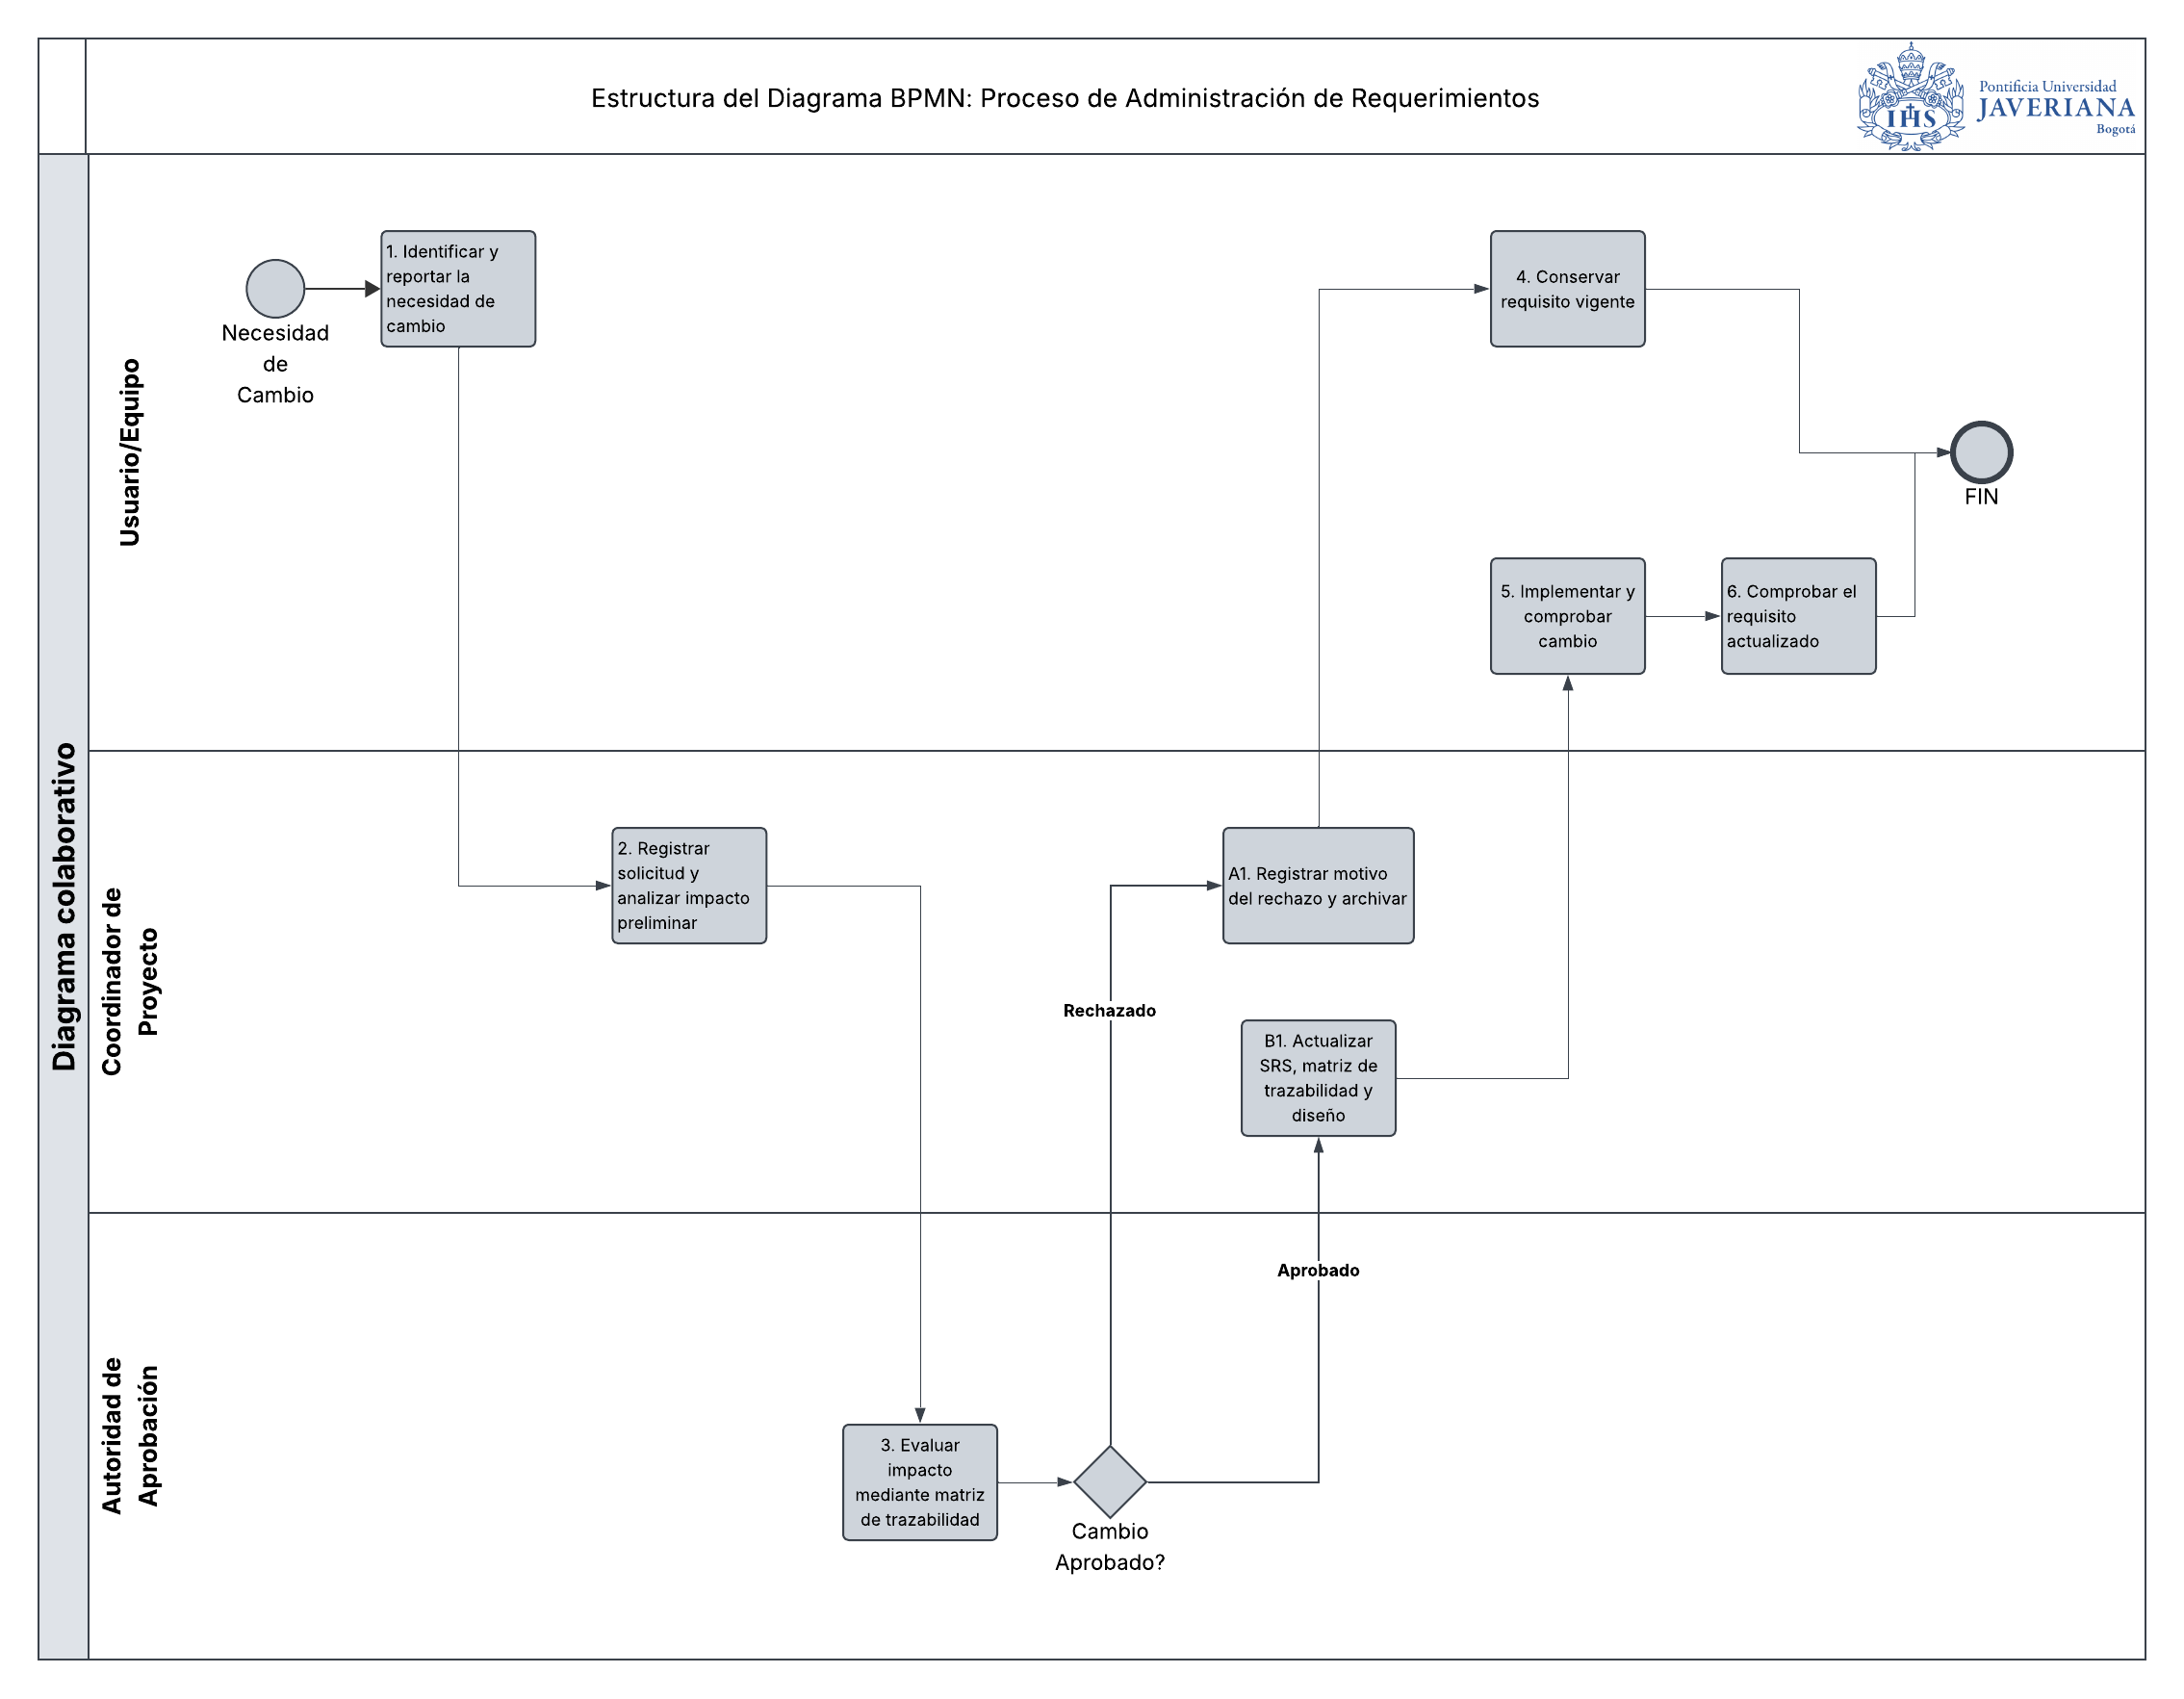
\includegraphics[width=1.18\textwidth]{figura_requerimientos.png}
    \caption{Proceso de administración de requerimientos y control de cambios. Fuente: elaboración propia.}
    \label{fig:bpmn-requerimientos}
\end{figure}